\subsubsection{Gamecontroller Implementering}

\noindent GameControlleren er det centrale komponent i game enginen, denne er ansvarlig 
for kommunikation til frontend del af applikationen. I denne implementering af 
GameControlleren har den adgang til alle spillet funktionaliteter gennem dennes
association til Combatcontroller, se \autoref{fig:CoreClassDiagram}, og BackendController
, som ikke er vist på \autoref{fig:CoreClassDiagram}.

Fra et implementering perspektiv er dette en nem løsning for en lille applikationen som denne
men fra et design perspektiv er dette en dårlig løsning. GameControlleren har alt for mange
grunde til at ændre sig og følger næppe SOLID principperne. \\

GameControlleren saver og loader spillet gennem sin relation til BackendController. 
Desværre er load funktionen ret kompliceret og burde være delt op i mindre functioner.
Source code for load kan ses på \autoref{fig:LoadFunction}

Koden bliver kompliceret idet den forsøger at gennemløbe alle Room objects i spillet
for på korrektvis at fjerne enemies og items, som allerede er blevet samlet op tidligere.
Her gennemløbes alle Room objects og i hvert room gennemløbes alle items i Room chest
objectet for at krydsreferer alle items med inventory listen for at se om de skal fjernes
som en del af save gamet.

Ligeledes håndtere den enemies og krydsreferer alle enemies med slainEnemies listen for at
se hvilke enemies spilleren allerede har besejret. Disse enemies fjerne herefter fra spillet.

\begin{figure}[H]
  \centering
  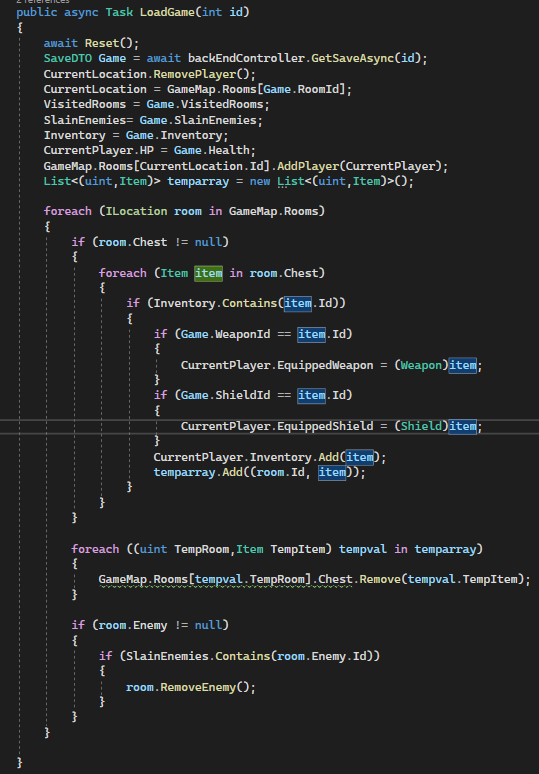
\includegraphics[]{02-Body/Implementering/GameEngineImplementering/Images/LoadFunction.png}
    \caption{Load funktionen, resetter game, setter de rigtige states og gennemløber
           alle Room instances og sætter deres state til den korrekte state.}
  \label{fig:LoadFunction}
\end{figure}


